%!TEX root = ../2019_7_Ozgumus_Semsi_Yigit.tex

\begingroup

This chapter presents the performance of all the models introduced in this thesis including 
the state of the art gan based anomaly detection methods (see section \ref{sec:gan_based_sota}) and 
the proposed model SENCEBGAN which is introduced on chapter \ref{chap:arim}. All experiments were run on 
a server containing Titan X. In particular, we will investigate the AUROC scores of the models with their 
corresponding precision and recall capacities across different cases. 

Organization of this chapter as follows: Section \ref{sec:exp_settings} gives a detailed explanation 
of the experimental setting providing obtaining the training and testing data and configurations of 
the models. Section \ref{sec:perf_metric} introduces the performance metrics that are used to evaluate 
and compare the models. Following two sections, section \ref{sec:exp_pure_gan} and 
\ref{sec:exp_sencebgan} describe the experiments conducted on the state of the art models and 
proposed model. Finally, section \ref{sec:exp_discuss} discusses the results of the experiments.


\section{Experiment Settings}
\label{sec:exp_settings}
Training and testing data for the experiments are obtained from the SEM image dataset \cite{sem}. 
Dataset contains 5 normal image samples with the resolution of $1024 \times 696$ and 40 Anomalous 
images samples (same resolution) with a corresponding mask image that denotes where each anomalous 
region is located. Training dataset is created by cropping $32 \times 32$ patches randomly from 
the normal images. Test dataset is obtained using the same method but with an overlapping sequential 
approach instead of randomization. Smaller patch size ($28 \times 28$) is also tested for preliminary 
gan experiments. Due to its size, designed generator network has one less combined transposed 
convolution layer (Transposed Convolution + Batch Normalization + Leaky ReLu) and some of the models 
we introduced in chapter \ref{chap:sota} were designed for minimum $32 \times 32$ images. Therefore 
$32 \times 32$ image patches are used throughout the experiments.
 
For all experiments, same hyper parameter values regarding the optimizer used in the training are used 
for all models. In terms of training, batch size and number of epochs are also fixed to equally 
measure the learning capacity of the generator discriminator networks contained in the models. Other 
related hyper parameter selections will be mentioned in their respective sections throughout this chapter.

\section{Performance Metrics}
\label{sec:perf_metric}
This section will introduce the performance metrics used for the interpretation of the experiments performed.
These are:
\begin{itemize}
	\item Precision
	\item Recall
	\item F1 Score
	\item AUROC (Area Under Receiver Operating Characteristic curve)
\end{itemize}

To define these performance metrics, first the statistical measures used in  classification problems  
will be introduced. Suppose we have a classification problem with a certain dataset. In this problem we 
have a condition or a feature we want to identify and in general some part of the dataset has 
this condition and the remaining part does not. If the prediction regarding to this condition is correct 
for the sample this is called \textbf{true positive}.\textbf{Sensitivity} measures the true positive rate in a 
classification problem. Same as the positive, \textbf{true negative} is correct rejection of the condition. 
\textbf{Specifity} is therefore described as the proportion of the true negative samples that are correctly 
rejected by the classification. There are 2 types of errors defined in this context. \textbf{Type 1} 
error refers to the rate of falsely identifying a negative sample as positive. It is also called the 
\textbf{false positive rate}. \textbf{Type 2} error measures the error rate of false rejections of the 
positive samples which is also defined as the \textbf{false negative rate}. Our performance measures are 
composed of these primal statistical measures. 

\textbf{Recall} is the ability of a model to find all the relevant cases within a dataset. In our case, 
detection of all the anomalous examples contained in the test set would indicate a perfect recall. Its 
score range is $[0,1]$ inclusive. Increasing recall capacity decreases the false negative rate to 
correctly identify all possible target class samples. \textbf{Precision} on the other hand is the 
ability of a classification model to identify \textbf{only} the relevant data points. Increased precision 
means a decrease in the false positive rate because a system favors precision aim towards eliminating all 
false predictions. The calculation of the both metrics is given below
\begin{align}
\textbf{recall} & = \frac{\text{true positives}}{\text{true positives} + \text{false negatives}} \\[5pt]
\textbf{precision} & = \frac{\text{true positives}}{\text{true positives} + \text{false positives}}
\end{align}

Precision and recall comprises a trade off situation. If the model favors the precision, the recall capacity
decreases because eliminating the false positives inadvertently increases the false negative rate and 
vice versa. To give equal importance to both metrics, \textbf{F1 score} is used. The F1 score is the 
harmonic mean of precision and recall taking both metrics into account in the following equation:
\begin{equation}
\text{F}_{1} = 2 \times \frac{\text{precision} \times \text{recall}}{\text{precision} + \text{recall}}
\end{equation}

The main metric we use to interpret the model performance is area under receiver operating characteristic 
curve, \textbf{AUROC} for short. 
\begin{figure}[h!]%
	\centering
	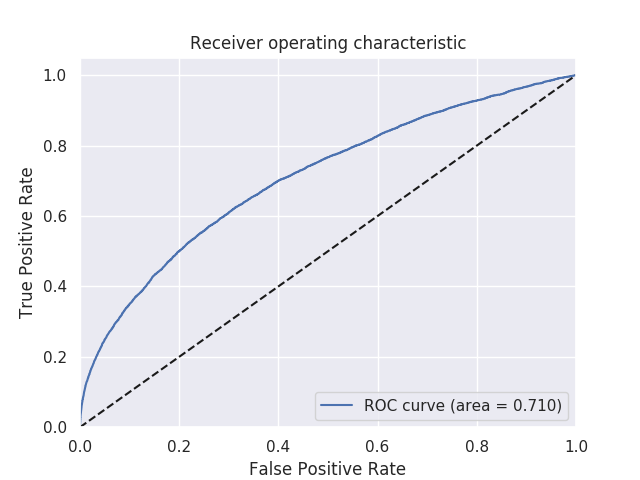
\includegraphics[width=0.8\textwidth]{expres/roc_curve}
	\caption{ROC Curve Example with AUROC value}
	\label{fig:roc_curve}%
\end{figure}
ROC curve visualizes the trade of relationship between the recall and precision capacity as the threshold for 
identifying a positive in the model changes. The threshold is the indicator value above which a sample is considered in the 
positive class. In our problem, threshold is determined from the anomaly score. ROC curve plots the true positive rate 
on the y-axis versus the false positive rate on the x-axis. (See figure \ref{fig:roc_curve})
True positive rate is actually recall. False positive rate is the probability of false detection for the system. 
Calculations for these rates are provided below:
\begin{align}
\textbf{True Positive Rate} & = \frac{\text{true positives}}{\text{true positives} + \text{false negatives}} \\[5pt]
\textbf{False Positive Rate} & = \frac{\text{false positives}}{\text{true negatives} + \text{false positives}}
\end{align}

the AUROC value can be obtained by calculating the area under the ROC curve which has a range between 0 and 1 
with a higher number indicating better classification performance.

In the performed experiments, AUROC value is considered as the main comparison metric amongst the models. 
Recall and precision are used to give an auxiliary information about the model's prediction accuracy and capacity. 
As a reporting criterion, highest F1 score obtained from the percentile interval between $80\%$ and $99.9\%$ is 
as a threshold is used to determine the optimal precision and recall values. 

\section{State of the Art GAN Based Model Experiments}
\label{sec:exp_pure_gan}
This section is devoted to the performance analysis of pure GAN based models. In the initial experiment stage, 
all state of the art GAN based models are implemented using the same generator and discriminator architecture. 
Since all the models are tested on known benchmark datasets and there is no experiment with our dataset, all models' 
initial run is acquired as a baseline. Baseline performances are reported in the table \ref{tab:exp_baseline}.

\begin{longtable}[c]{|c|cccc|}
	\caption{Baseline performance values of the state of the art GAN based models}
	\label{tab:exp_baseline}\\
	\hline
	\multirow{2}{*}{\textbf{Models}} & \multicolumn{4}{c|}{\textbf{Metrics}} \\ \cline{2-5} 
	& AUROC & Precision & Recall & F1 Score \\ \hline
	\endhead
	%
 \multicolumn{1}{|c|}{AnoGAN} & \multicolumn{1}{c}{0.59941} & \multicolumn{1}{c}{0.14253} & \multicolumn{1}{c}{0.27783} & \multicolumn{1}{c|}{0.18841} \\ \hline
\multicolumn{1}{|c|}{BiGAN} & \multicolumn{1}{c}{0.62699} & \multicolumn{1}{c}{0.10201} & \multicolumn{1}{c}{0.32227} & \multicolumn{1}{c|}{0.15497} \\ \hline
\multicolumn{1}{|c|}{ALAD} & \multicolumn{1}{c}{0.44842} & \multicolumn{1}{c}{0.05521} & \multicolumn{1}{c}{0.17443} & \multicolumn{1}{c|}{0.08388} \\ \hline
\multicolumn{1}{|c|}{GANomaly} & \multicolumn{1}{c}{0.77697} & \multicolumn{1}{c}{0.39701} & \multicolumn{1}{c}{0.31356} & \multicolumn{1}{c|}{0.35038} \\ \hline
\multicolumn{1}{|c|}{Skip-GANomaly} & \multicolumn{1}{c}{0.53182} & \multicolumn{1}{c}{0.07379} & \multicolumn{1}{c}{0.23314} & \multicolumn{1}{c|}{0.11211} \\ \hline
\end{longtable}

After this initial test, it is observed that pure GAN based models performed poorly on our target dataset and 
only GANomaly model obtained a full precision/recall curve even though it is below $0.5$. Precision recall 
curve is an alternative way of visualizing the precision and recall capacity of a model. The definition of 
precision states that if the number of predictions are equal to the number of anomalies contained in the dataset then the 
precision is exactly $1.0$. In order for that to be happen, model should not make a prediction unless it is 
absolutely certain hence with this criterion in mind the model has an greater false negative rate. So if the 
precision is $1.0$ that means with a given threshold the model (acceptance point such that if sample has a greater or equal score than threshold it is considered as anomaly) can always make the right prediction. From the 
perspective of recall, it also means that there is a threshold value that enables model to find all anomalies 
contained in the dataset even if it increases the overall false positive rate of prediction performance.  

\begin{table}[!h]
	\centering
	\caption{Ablation study for AnoGAN to test the effect of various training improvements for stabilization.}
	\label{tab:anogan_ablation}
	\resizebox{\textwidth}{!}{%
		\begin{tabular}{|c|l|llll|}
			\hline
			\multicolumn{2}{|c|}{\multirow{2}{*}{\textbf{Model}}} & \multicolumn{4}{c|}{\textbf{Metrics}} \\ \cline{3-6} 
			\multicolumn{2}{|c|}{} & AUROC & \multicolumn{1}{c}{Precision} & \multicolumn{1}{c}{Recall} & \multicolumn{1}{c|}{F1 Score} \\ \hline
			\multirow{8}{*}{AnoGAN} & Normal & \multicolumn{1}{c}{0.59941} & \multicolumn{1}{c}{\textbf{0.14253}} & \multicolumn{1}{c}{0.27783} & \multicolumn{1}{c|}{0.18841} \\ \cline{2-6} 
			& IN & \multicolumn{1}{c}{0.59978} & \multicolumn{1}{c}{0.14010} & \multicolumn{1}{c}{0.27309} & \multicolumn{1}{c|}{0.18512} \\ \cline{2-6} 
			& SL & \multicolumn{1}{c}{0.43092} & \multicolumn{1}{c}{0.06875} & \multicolumn{1}{c}{0.13401} & \multicolumn{1}{c|}{0.09087} \\ \cline{2-6} 
			& LF & \multicolumn{1}{c}{0.43319} & \multicolumn{1}{c}{0.06822} & \multicolumn{1}{c}{0.17732} & \multicolumn{1}{c|}{0.09854} \\ \cline{2-6} 
			& IN + SL & \multicolumn{1}{c}{\textbf{0.59987}} & \multicolumn{1}{c}{0.12877} & \multicolumn{1}{c}{\textbf{0.33468}} & \multicolumn{1}{c|}{\textbf{0.18958}} \\ \cline{2-6} 
			& IN + LF & \multicolumn{1}{c}{0.52329} & \multicolumn{1}{c}{0.09075} & \multicolumn{1}{c}{0.23587} & \multicolumn{1}{c|}{0.13107} \\ \cline{2-6} 
			& SL + LF & \multicolumn{1}{c}{0.53469} & \multicolumn{1}{c}{0.09440} & \multicolumn{1}{c}{0.24534} & \multicolumn{1}{c|}{0.13634} \\ \cline{2-6} 
			& LF + SL + IN & \multicolumn{1}{c}{0.54625} & \multicolumn{1}{c}{0.09973} & \multicolumn{1}{c}{0.25922} & \multicolumn{1}{c|}{0.14405} \\ \hline	
		\end{tabular}%
	}
\end{table}

In the ablation studies, mainly 3 heuristic improvements are tested to improve the stabilization of the 
training and consequently improve the performance. These are:
\begin{itemize}
	\item {(IN) Inclusion of noise to the real input images and generated images before feeding them into 
		discriminator network to confuse discriminator. }
	\item {(SL) Using soft labels for the class representation instead of hard 0,1 labeling for the cross 
		entropy computation used in the adversarial loss}
	\item {(LF) Flipping labels of the samples that are fed to the discriminator. Since the discriminator 
		knows the type of image provided to it, mixing the labels 
	helps to confuse discriminator so that gradient flow to the generator does not decrease.}
\end{itemize}

In the ablation study of AnoGAN (see table \ref{tab:anogan_ablation}), overall performance couldn't pass 
the $0.6$ mark. Addition of the noise and using soft labels improved the overall score by a small margin but 
decreased the precision capacity of the model. Recall capacity is slightly improved with the addition of noise 
and soft labelling. Using label flipping and soft labelling alone did not contribute any improvement on the 
contrary it pulled down the AUROC value below $0.5$. Separation histogram, precision/recall trade-off and 
ROC curve of the best configuration is provided in figure \ref{fig:exp_ext_anogan}.

\begin{figure}[h!]
	\def\tabularxcolumn#1{m{#1}}
	\begin{tabularx}{\linewidth}{@{}XXX@{}}
		\begin{tabular}{ccc}
			\subfloat[Separation Histogram]{\includegraphics[width=0.3\textwidth]{expres/anogan/hist}} 
			& \subfloat[Precision/Recall Trade off]{\includegraphics[width=0.3\textwidth]{expres/anogan/prc}} &
			\subfloat[ROC Curve]{\includegraphics[width=0.3\textwidth]{expres/anogan/roc}}
		\end{tabular}
	\end{tabularx}
	\caption{Visual performance analysis info for the best configuration of ablation study of AnoGAN}\label{fig:exp_ext_anogan}
\end{figure}

Table \ref{tab:bigan_ablation} shows the ablation study for the BiGAN model. We observe that baseline 
performance is only marginally improved by the addition of noise and label flipping. Single heuristic 
additions considerably made worse the overall performance with the exception of using soft class labels. 
Another aspect about the general performance is that even though its AUROC performance is higher than 
AnoGAN, precision of the model achieved a lower score while improving its total recall value. 

\begin{table}[!h]
	\centering
	\caption{Ablation study for BiGAN to test the effect of various training improvements for stabilization.}
	\label{tab:bigan_ablation}
	\resizebox{\textwidth}{!}{%
		\begin{tabular}{|c|l|llll|}
			\hline
			\multicolumn{2}{|c|}{\multirow{2}{*}{\textbf{Model}}} & \multicolumn{4}{c|}{\textbf{Metrics}} \\ \cline{3-6} 
			\multicolumn{2}{|c|}{} & AUROC & \multicolumn{1}{c}{Precision} & \multicolumn{1}{c}{Recall} & \multicolumn{1}{c|}{F1 Score} \\ \hline
			\multirow{8}{*}{BiGAN} & Normal & \multicolumn{1}{c}{0.62699} & \multicolumn{1}{c}{0.10201} & \multicolumn{1}{c}{0.32227} & \multicolumn{1}{c|}{0.15497} \\ \cline{2-6} 
			& IN & \multicolumn{1}{c}{0.38195} & \multicolumn{1}{c}{0.03721} & \multicolumn{1}{c}{0.11756} & \multicolumn{1}{c|}{0.05653} \\ \cline{2-6} 
			& SL & \multicolumn{1}{c}{0.58904} & \multicolumn{1}{c}{0.08251} & \multicolumn{1}{c}{0.26066} & \multicolumn{1}{c|}{0.12534} \\ \cline{2-6} 
			& LF & \multicolumn{1}{c}{0.39541} & \multicolumn{1}{c}{0.03532} & \multicolumn{1}{c}{0.11160} & \multicolumn{1}{c|}{0.05366} \\ \cline{2-6} 
			& IN + SL & \multicolumn{1}{c}{0.52646} & \multicolumn{1}{c}{0.06978} & \multicolumn{1}{c}{0.22045} & \multicolumn{1}{c|}{0.10600} \\ \cline{2-6} 
			& IN + LF & \multicolumn{1}{c}{\textbf{0.63362}} & \multicolumn{1}{c}{\textbf{0.10917}} & \multicolumn{1}{c}{\textbf{0.34490}} & \multicolumn{1}{c|}{\textbf{0.16585}} \\ \cline{2-6} 
			& SL + LF & \multicolumn{1}{c}{0.57855} & \multicolumn{1}{c}{0.08483} & \multicolumn{1}{c}{0.26800} & \multicolumn{1}{c|}{0.12887} \\ \cline{2-6} 
			& LF + SL + IN & \multicolumn{1}{c}{0.62912} & \multicolumn{1}{c}{0.10617} & \multicolumn{1}{c}{0.33542} & \multicolumn{1}{c|}{0.16129} \\ \hline
		\end{tabular}%
	}
\end{table}

Considering the whole capacity of the model, we observe in figure \ref{fig:exp_ext_bigan} that the highest 
capacity and recall values along the threshold axis decreased considerably. 


\begin{figure}[h!]
	\def\tabularxcolumn#1{m{#1}}
	\begin{tabularx}{\linewidth}{@{}XXX@{}}
		\begin{tabular}{ccc}
			\subfloat[Separation Histogram]{\includegraphics[width=0.3\textwidth]{expres/bigan/hist}} 
			& \subfloat[Precision/Recall Trade off]{\includegraphics[width=0.3\textwidth]{expres/bigan/prc}} &
			\subfloat[ROC Curve]{\includegraphics[width=0.3\textwidth]{expres/bigan/roc}}
		\end{tabular}
	\end{tabularx}
	\caption{Visual performance analysis info for the best configuration of ablation study of BiGAN}\label{fig:exp_ext_bigan}
\end{figure}

Figure \ref{fig:expres_recs_bigan} shows the reconstructions of given input images during the 
training. Convergence issue mentioned in section \ref{sec:conv_enc} supports the results provided 
here as can be seen from the training progression, there is no visual resemblance between 
the input images and their corresponding reconstructions.

\begin{figure}[!ht]	
	\setlength\tabcolsep{1pt}
	\settowidth\rotheadsize{Reconstructions}
	\begin{tabularx}{\linewidth}{l XXXXXX}
		\rothead{Image Samples}  & \includegraphics[width=0.16\textwidth,valign=m]{expres/bigan/ims/input_0}
		& \includegraphics[width=0.16\textwidth,valign=m]{expres/bigan/ims/input_10}
		& \includegraphics[width=0.16\textwidth,valign=m]{expres/bigan/ims/input_20}
		& \includegraphics[width=0.16\textwidth,valign=m]{expres/bigan/ims/input_30}
		& \includegraphics[width=0.16\textwidth,valign=m]{expres/bigan/ims/input_40}
		& \includegraphics[width=0.16\textwidth,valign=m]{expres/bigan/ims/input_50} \\
		\rothead{Reconstructions} & \includegraphics[width=0.16\textwidth,valign=m]{expres/bigan/ims/rec_0}
		& \includegraphics[width=0.16\textwidth,valign=m]{expres/bigan/ims/rec_10} 
		& \includegraphics[width=0.16\textwidth,valign=m]{expres/bigan/ims/rec_20} 
		& \includegraphics[width=0.16\textwidth,valign=m]{expres/bigan/ims/rec_30} 
		& \includegraphics[width=0.16\textwidth,valign=m]{expres/bigan/ims/rec_40} 
		&\includegraphics[width=0.16\textwidth,valign=m]{expres/bigan/ims/rec_50}
	\end{tabularx}
	\caption{Reconstruction examples from BiGAN model training with best configuration (Epochs 1,10,20,30,40 and 50)}\label{fig:expres_recs_bigan}
\end{figure}

Ablation study for ALAD model is presented in table \ref{tab:alad_ablation}. Unlike AnoGAN 
and BiGAN, ALAD couldn't pass the $0.5$ mark performance on its own. Using heuristics to 
improve the training proved useful in this model as the configuration with the best performance 
is the one with all three heuristics combined. Even with this boost, the model's precision and recall
capacity is fairly limited as can be seen from the trade off graph in Figure \ref{fig:exp_ext_alad}. 
Even with the highest value of the threshold does not provide a precision above $50\%$. 

\begin{table}[!h]
	\centering
	\caption{Ablation study for ALAD to test the effect of various training improvements for stabilization.}
	\label{tab:alad_ablation}
	\resizebox{\textwidth}{!}{%
		\begin{tabular}{|c|l|llll|}
			\hline
			\multicolumn{2}{|c|}{\multirow{2}{*}{\textbf{Model}}} & \multicolumn{4}{c|}{\textbf{Metrics}} \\ \cline{3-6} 
			\multicolumn{2}{|c|}{} & AUROC & \multicolumn{1}{c}{Precision} & \multicolumn{1}{c}{Recall} & \multicolumn{1}{c|}{F1 Score} \\ \hline
			\multirow{8}{*}{ALAD} & Normal & \multicolumn{1}{c}{0.44842} & \multicolumn{1}{c}{0.05521} & \multicolumn{1}{c}{0.17443} & \multicolumn{1}{c|}{0.08388} \\ \cline{2-6} 
			& IN & \multicolumn{1}{c}{0.49447} & \multicolumn{1}{c}{0.06171} & \multicolumn{1}{c}{0.19385} & \multicolumn{1}{c|}{0.09321} \\ \cline{2-6} 
			& SL & \multicolumn{1}{c}{0.52920} & \multicolumn{1}{c}{\textbf{0.07854}} & \multicolumn{1}{c}{\textbf{0.24812}} & \multicolumn{1}{c|}{\textbf{0.11931}} \\ \cline{2-6} 
			& LF & \multicolumn{1}{c}{0.55545} & \multicolumn{1}{c}{0.07326} & \multicolumn{1}{c}{0.23146} & \multicolumn{1}{c|}{0.11130} \\ \cline{2-6} 
			& IN + SL & \multicolumn{1}{c}{0.48488} & \multicolumn{1}{c}{0.05918} & \multicolumn{1}{c}{0.18697} & \multicolumn{1}{c|}{0.08990} \\ \cline{2-6} 
			& IN + LF & \multicolumn{1}{c}{0.52712} & \multicolumn{1}{c}{0.06450} & \multicolumn{1}{c}{0.20379} & \multicolumn{1}{c|}{0.09799} \\ \cline{2-6} 
			& SL + LF & \multicolumn{1}{c}{0.49057} & \multicolumn{1}{c}{0.06441} & \multicolumn{1}{c}{0.20348} & \multicolumn{1}{c|}{0.09784} \\ \cline{2-6} 
			& LF + SL + IN & \multicolumn{1}{c}{\textbf{0.55904}} & \multicolumn{1}{c}{0.07588} & \multicolumn{1}{c}{0.23971} & \multicolumn{1}{c|}{0.11527} \\ \hline
		\end{tabular}%
	}
\end{table}

Figure \ref{fig:expres_recs_alad} shows the reconstruction capability of ALAD during training. 
Same as BiGAN, it suffers from the encoder, generator convergence problem. There is no apparent 
visual resemblance between the input and the corresponding reconstructions. 

\begin{figure}[h!]
	\def\tabularxcolumn#1{m{#1}}
	\begin{tabularx}{\linewidth}{@{}XXX@{}}
		\begin{tabular}{ccc}
			\subfloat[Separation Histogram]{\includegraphics[width=0.3\textwidth]{expres/alad/hist}} 
			& \subfloat[Precision/Recall Trade off]{\includegraphics[width=0.3\textwidth]{expres/alad/prc}} &
			\subfloat[ROC Curve]{\includegraphics[width=0.3\textwidth]{expres/alad/roc}}
		\end{tabular}
	\end{tabularx}
	\caption{Visual performance analysis info for the best configuration of ablation study of ALAD}\label{fig:exp_ext_alad}
\end{figure}

\begin{figure}[!ht]	
	\setlength\tabcolsep{1pt}
	\settowidth\rotheadsize{Reconstructions}
	\begin{tabularx}{\linewidth}{l XXXXXX}
		\rothead{Image Samples}  & \includegraphics[width=0.16\textwidth,valign=m]{expres/alad/ims/input_0}
		& \includegraphics[width=0.16\textwidth,valign=m]{expres/alad/ims/input_10}
		& \includegraphics[width=0.16\textwidth,valign=m]{expres/alad/ims/input_20}
		& \includegraphics[width=0.16\textwidth,valign=m]{expres/alad/ims/input_30}
		& \includegraphics[width=0.16\textwidth,valign=m]{expres/alad/ims/input_40}
		& \includegraphics[width=0.16\textwidth,valign=m]{expres/alad/ims/input_50} \\
		\rothead{Reconstructions} & \includegraphics[width=0.16\textwidth,valign=m]{expres/alad/ims/rec_0}
		& \includegraphics[width=0.16\textwidth,valign=m]{expres/alad/ims/rec_10} 
		& \includegraphics[width=0.16\textwidth,valign=m]{expres/alad/ims/rec_20} 
		& \includegraphics[width=0.16\textwidth,valign=m]{expres/alad/ims/rec_30} 
		& \includegraphics[width=0.16\textwidth,valign=m]{expres/alad/ims/rec_40} 
		&\includegraphics[width=0.16\textwidth,valign=m]{expres/alad/ims/rec_50}
	\end{tabularx}
	\caption{Reconstruction examples from ALAD model training with best configuration (Epochs 1,10,20,30,40 and 50)}\label{fig:expres_recs_alad}
\end{figure}

In table \ref{tab:ganomaly_ablation} we present the performance results for GANomaly. Since it is 
not a pure gan based model (along with Skip-GANomaly) their performance measure is not used as a comparison 
for the proposed model. However ablation study is performed to measure the impact of general performance 
because our proposed model procured its secondary encoder network with the initial intuition that the 
latent representation based anomaly detection score performs better than image space in GANomaly architecture. 

\begin{table}[!h]
	\centering
	\caption{Ablation study for GANomaly to test the effect of various training improvements for stabilization. }
	\label{tab:ganomaly_ablation}
	\resizebox{\textwidth}{!}{%
		\begin{tabular}{|c|l|llll|}
			\hline
			\multicolumn{2}{|c|}{\multirow{2}{*}{\textbf{Model}}} & \multicolumn{4}{c|}{\textbf{Metrics}} \\ \cline{3-6} 
			\multicolumn{2}{|c|}{} & AUROC & \multicolumn{1}{c}{Precision} & \multicolumn{1}{c}{Recall} & \multicolumn{1}{c|}{F1 Score} \\ \hline
			\multirow{8}{*}{GANomaly} & Normal & \multicolumn{1}{c}{\textbf{0.77697}} & \multicolumn{1}{c}{\textbf{0.39701}} & \multicolumn{1}{c}{0.31356} & \multicolumn{1}{c}{\textbf{0.35038}} \\ \cline{2-6} 
			& IN & \multicolumn{1}{c}{0.63222} & \multicolumn{1}{c}{0.09891} & \multicolumn{1}{c}{0.31249} & \multicolumn{1}{c|}{0.15266} \\ \cline{2-6} 
			& SL & \multicolumn{1}{c}{0.75224} & \multicolumn{1}{c}{0.35288} & \multicolumn{1}{c}{0.27870} & \multicolumn{1}{c|}{0.31143} \\ \cline{2-6} 
			& LF & \multicolumn{1}{c}{0.76225} & \multicolumn{1}{c}{0.37611} & \multicolumn{1}{c}{0.29704} & \multicolumn{1}{c|}{0.33193} \\ \cline{2-6} 
			& IN + SL & \multicolumn{1}{c}{0.62626} & \multicolumn{1}{c}{0.09693} & \multicolumn{1}{c}{0.30622} & \multicolumn{1}{c|}{0.14725} \\ \cline{2-6} 
			& IN + LF & \multicolumn{1}{c}{0.64009} & \multicolumn{1}{c}{0.10496} & \multicolumn{1}{c}{\textbf{0.33160}} & \multicolumn{1}{c|}{0.15945} \\ \cline{2-6} 
			& SL + LF & \multicolumn{1}{c}{0.76342} & \multicolumn{1}{c}{0.37495} & \multicolumn{1}{c}{0.29613} & \multicolumn{1}{c|}{0.33091} \\ \cline{2-6} 
			& LF + SL + IN & \multicolumn{1}{c}{0.63179} & \multicolumn{1}{c}{0.09548} & \multicolumn{1}{c}{0.30163} & \multicolumn{1}{c|}{0.14504} \\ \hline
		\end{tabular}%
	}
\end{table}

Experiments for GANomaly shows that heuristics aimed to improve the GAN stabilization didn't 
improve the AUROC value obtained from the baseline performance. One can conclude that because of 
the generator is created from an autoencoder architecture, there is not a convergence issue 
which observed on the pure GAN based models. As figure \ref{fig:exp_ext_ganomaly} shows, the 
separation histogram and precision/recall trade off presents a significantly better results compared 
to the prior ablation study results. 

\begin{figure}[h!]
	\def\tabularxcolumn#1{m{#1}}
	\begin{tabularx}{\linewidth}{@{}XXX@{}}
		\begin{tabular}{ccc}
			\subfloat[Separation Histogram]{\includegraphics[width=0.3\textwidth]{expres/ganomaly/hist}} 
			& \subfloat[Precision/Recall Trade off]{\includegraphics[width=0.3\textwidth]{expres/ganomaly/prc}} &
			\subfloat[ROC Curve]{\includegraphics[width=0.3\textwidth]{expres/ganomaly/roc}}
		\end{tabular}
	\end{tabularx}
	\caption{Visual performance analysis info for the best configuration of ablation study of GANomaly}\label{fig:exp_ext_ganomaly}
\end{figure}


Table \ref{tab:sganomaly_ablation} shows the ablation study on the Skip-GANomaly model. All the 
combinations of heuristics marginally improved the overall AUROC performance. Despite noise inclusion 
obtained the best AUROC score, its combination with label flipping obtain a fairly close score with a slightly 
higher F1 score. 
\begin{table}[!h]
	\centering
	\caption{Ablation study for Skip-GANomaly to test the effect of various training improvements for stabilization.}
	\label{tab:sganomaly_ablation}
	\resizebox{\textwidth}{!}{%
		\begin{tabular}{|c|l|llll|}
			\hline
			\multicolumn{2}{|c|}{\multirow{2}{*}{\textbf{Model}}} & \multicolumn{4}{c|}{\textbf{Metrics}} \\ \cline{3-6} 
\multicolumn{2}{|c|}{} & AUROC & \multicolumn{1}{c}{Precision} & \multicolumn{1}{c}{Recall} & \multicolumn{1}{c|}{F1 Score} \\ \hline
\multirow{8}{*}{Skip-GANomaly} & Normal & \multicolumn{1}{c}{0.53182} & \multicolumn{1}{c}{0.07379} & \multicolumn{1}{c}{0.23314} & \multicolumn{1}{c|}{0.11211} \\ \cline{2-6} 
& IN & \multicolumn{1}{c}{\textbf{0.58120}} & \multicolumn{1}{c}{0.10646} & \multicolumn{1}{c}{0.25225} & \multicolumn{1}{c|}{0.14973} \\ \cline{2-6} 
& SL & \multicolumn{1}{c}{0.55309} & \multicolumn{1}{c}{0.08686} & \multicolumn{1}{c}{0.27442} & \multicolumn{1}{c|}{0.13196} \\ \cline{2-6} 
& LF & \multicolumn{1}{c}{0.53703} & \multicolumn{1}{c}{0.07617} & \multicolumn{1}{c}{0.24063} & \multicolumn{1}{c|}{0.11571} \\ \cline{2-6} 
& IN + SL & \multicolumn{1}{c}{0.57432} & \multicolumn{1}{c}{0.10156} & \multicolumn{1}{c}{0.24063} & \multicolumn{1}{c|}{0.14283} \\ \cline{2-6} 
& IN + LF & \multicolumn{1}{c}{0.58041} & \multicolumn{1}{c}{\textbf{0.12485}} & \multicolumn{1}{c}{0.19721} & \multicolumn{1}{c|}{\textbf{0.15290}} \\ \cline{2-6} 
& SL + LF & \multicolumn{1}{c}{0.55675} & \multicolumn{1}{c}{0.08749} & \multicolumn{1}{c}{\textbf{0.27641}} & \multicolumn{1}{c|}{0.13291} \\ \cline{2-6} 
& LF + SL + IN & \multicolumn{1}{c}{0.57402} & \multicolumn{1}{c}{0.10407} & \multicolumn{1}{c}{0.24659} & \multicolumn{1}{c|}{0.14637} \\ \hline
		\end{tabular}%
	}
\end{table}

From the separation table and the precision/ recall trade off, we can observe that even though the 
Skip-GANomaly model is fairly similar to the GANomaly architecture, its performance is not better than 
AnoGAN or BiGAN. We speculate that the main reason for this drop in the overall quality of the model is 
using image space to compute the anomaly score. 

\begin{figure}[h!]
	\def\tabularxcolumn#1{m{#1}}
	\begin{tabularx}{\linewidth}{@{}XXX@{}}
		\begin{tabular}{ccc}
			\subfloat[Separation Histogram]{\includegraphics[width=0.3\textwidth]{expres/anogan/hist}} 
			& \subfloat[Precision/Recall Trade off]{\includegraphics[width=0.3\textwidth]{expres/anogan/prc}} &
			\subfloat[ROC Curve]{\includegraphics[width=0.3\textwidth]{expres/anogan/roc}}
		\end{tabular}
	\end{tabularx}
	\caption{Visual performance analysis info for the best configuration of ablation study of Skip-GANomaly}\label{fig:exp_ext_sganomaly}
\end{figure}

These experiments and ablation studies are done to gain insight towards the answers of two 
major questions. 
\begin{itemize}
	\item {How does the GAN based anomaly 
		detection frameworks present in the literature perform using our dataset ?}
	\item {If they don't perform well, is there a way to modify the aspect of the model that 
		creates the problem to improve their performance ?}
\end{itemize}
Our observations of the experiment results and their interpretation drew a path regards to the methodology we 
need to follow and the issues we need to focus. Following experiments will explain 
this approach.


\section{Proposed Model Analysis}
\label{sec:exp_sencebgan}

This section presents the experiments for our proposed model. Our methodology breaks down to three steps.
\begin{itemize}
	\item { Stabilizing the GAN training}
	\item { Solving convergence problem of encoder network for inverse mapping}
	\item { Experiments targeted to improve the performance}
\end{itemize}

For the first step of the experimentation, energy based generative adversarial network is implemented 
and trained. The main focus of this experiment to observe whether generator network learns to create an 
artificial image which resembles the training data. Figure \ref{fig:ebgan_reconstruct} shows the 
reconstruction samples of the generator from the EBGAN training.

\begin{figure}[h!]
	\def\tabularxcolumn#1{m{#1}}
	\begin{tabularx}{\textwidth}{@{}XXXX@{}}
		\begin{tabular}{cccc}
			\includegraphics[width=0.25\textwidth]{expres/ebgan/ims/input_1}
			& \includegraphics[width=0.25\textwidth]{expres/ebgan/ims/input_2}
			& \includegraphics[width=0.25\textwidth]{expres/ebgan/ims/input_3}
			& 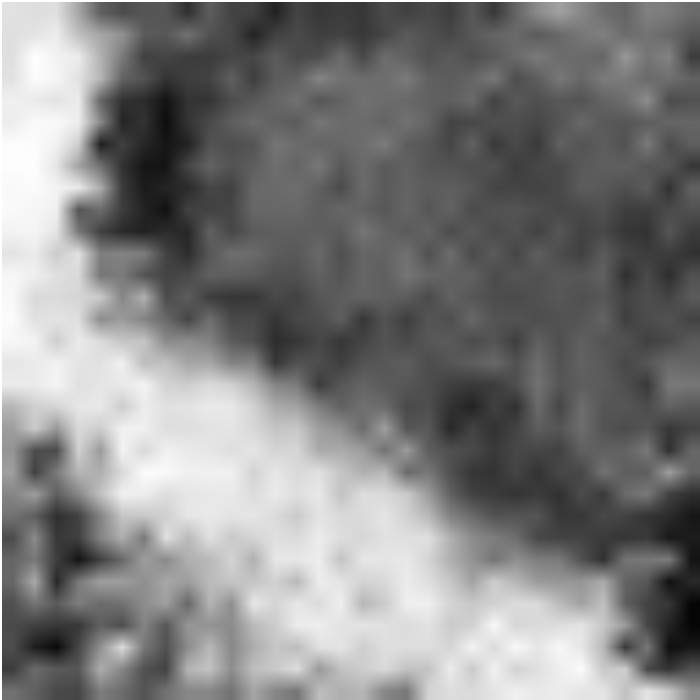
\includegraphics[width=0.25\textwidth]{expres/ebgan/ims/input_4}
		\end{tabular}
	\end{tabularx}
	\caption{Reconstruction samples from the EBGAN training}\label{fig:ebgan_reconstruct}
\end{figure}

Second stage of the experiments is for the addition of encoder network and its sequential training. 
ENCEBGAN model (see section \ref{sec:encebgan}) is proposed to observe the reconstruction quality and anomaly detection 
performance. Figure \ref{fig:encebgan_training} shows the training progression of the individual networks. 
Figure \ref{fig:encebgan_reconstruction} presents the reconstruction samples both from training and inference. First two columns 
are obtained from the training of encoder network during training. The last column is the reconstruction of an anomalous sample from 
the testing phase. 

\begin{figure}[h!]
	\def\tabularxcolumn#1{m{#1}}
	\begin{tabularx}{\linewidth}{@{}XXX@{}}
		\begin{tabular}{ccc}
			\subfloat[Generator Training Progression]{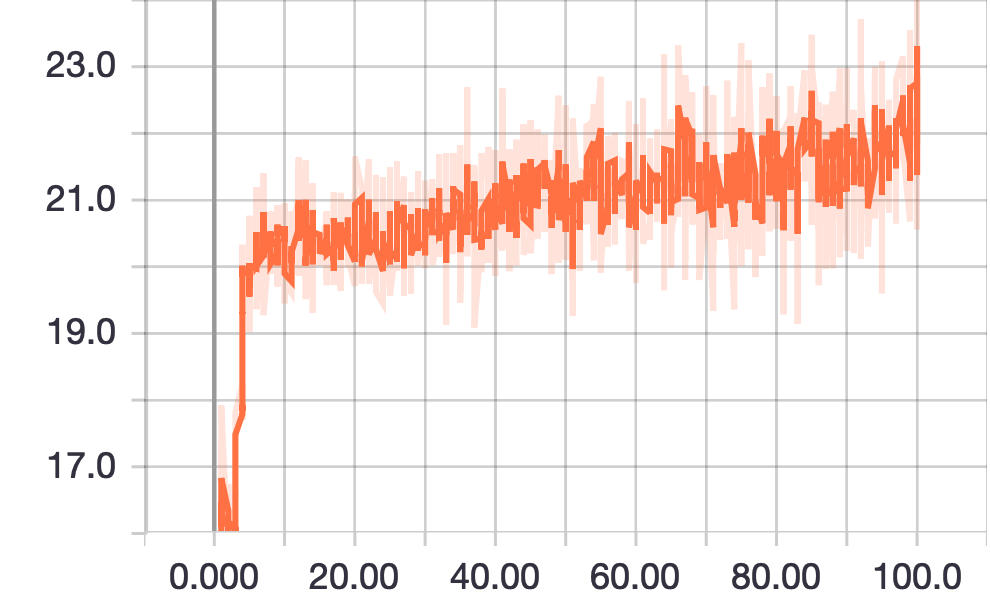
\includegraphics[width=0.3\textwidth]{expres/encebgan/encebgan_gen_loss}} 
			& \subfloat[Discriminator Training Progression]{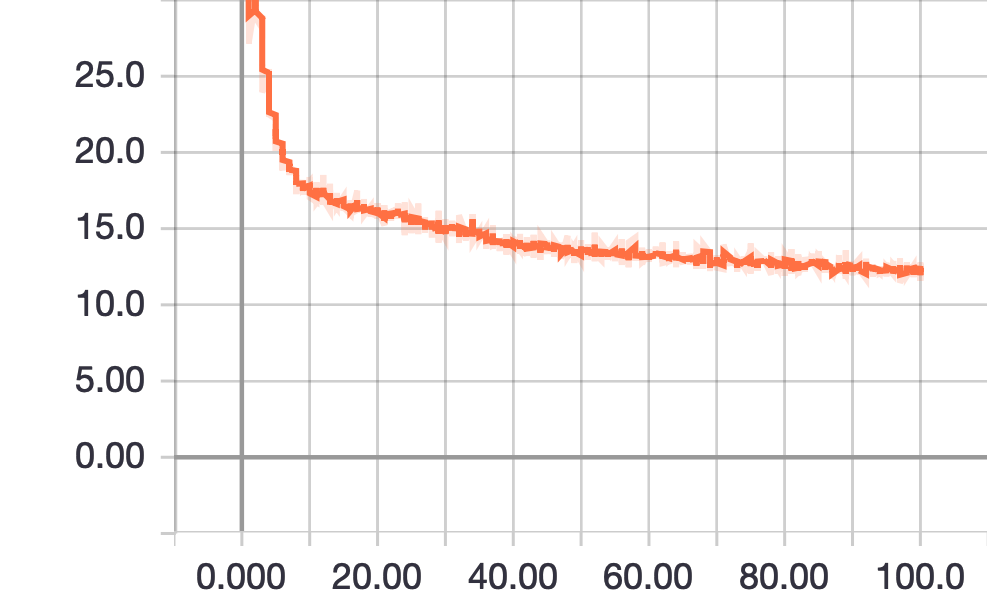
\includegraphics[width=0.3\textwidth]{expres/encebgan/encebgan_disc_loss}} &
			\subfloat[Encoder Training Progression]{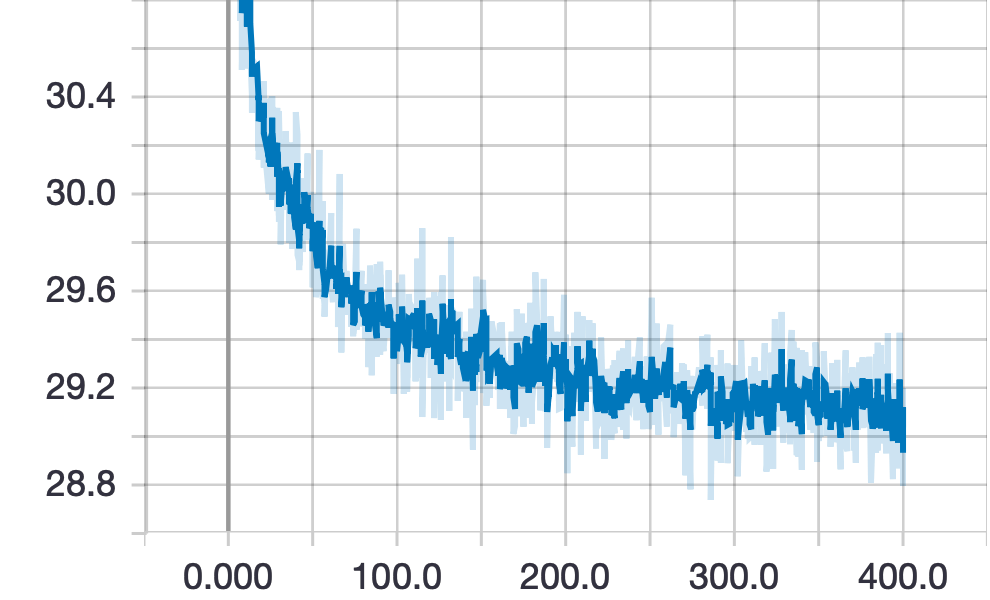
\includegraphics[width=0.3\textwidth]{expres/encebgan/encebgan_enc_loss}}
		\end{tabular}
	\end{tabularx}
	\caption{Training progression of ENCEBGAN model}\label{fig:encebgan_training}
\end{figure}

\begin{figure}[!h]	
	\setlength\tabcolsep{1pt}
	\settowidth\rotheadsize{Reconstructions}
	\begin{tabularx}{\linewidth}{l XXXX}
		\rothead{Image Samples}  & \includegraphics[width=0.25\textwidth,valign=m]{expres/encebgan/ims/input_1}
		& \includegraphics[width=0.25\textwidth,valign=m]{expres/encebgan/ims/input_2}
		& \includegraphics[width=0.25\textwidth,valign=m]{expres/encebgan/ims/input_3}
		& \includegraphics[width=0.25\textwidth,valign=m]{expres/encebgan/ims/input_4} \\
		\rothead{Reconstructions} & \includegraphics[width=0.25\textwidth,valign=m]{expres/encebgan/ims/rec_1}
		& \includegraphics[width=0.25\textwidth,valign=m]{expres/encebgan/ims/rec_2} 
		& \includegraphics[width=0.25\textwidth,valign=m]{expres/encebgan/ims/rec_3} 
		&\includegraphics[width=0.25\textwidth,valign=m]{expres/encebgan/ims/rec_4} \\
	\end{tabularx}
	\caption{Reconstruction examples of ENCEBGAN model obtained from both training and testing stage}\label{fig:encebgan_reconstruction}
\end{figure}

Last stage of the experiments focus on improving the overall performance of the model. As Figure 
\ref{fig:sencebgan_reconstruction} shows, the reconstruction power of ENCEBGAN and SENCEBGAN models 
are similar in terms of the retention of the filament structure and its noisy nature. Latent space 
based anomaly detection methods are investigated to mitigate the effect of reconstruction quality to 
performance. Figure \ref{fig:sencebgan_training} presents the training process of the final proposed 
model. In the first stage, generator and discriminator models are trained with adversarial approach. 
In the second stage $E_{G}$ (Generator Encoder) is trained using the fixed generator and discriminator 
networks. Finally in the third stage, $E_{R}$ (Reconstruction Encoder) is trained by encoding the inputs and 
their reconstructions.

\begin{figure}[h!]
	\def\tabularxcolumn#1{m{#1}}
	\begin{tabularx}{\linewidth}{@{}XXXX@{}}
		\begin{tabular}{cccc}
			\subfloat[Generator Training Progression]{\includegraphics[width=0.25\textwidth]{expres/sencebgan/sencebgan_gen_loss}} 
			& \subfloat[Discriminator Training Progression]{\includegraphics[width=0.25\textwidth]{expres/sencebgan/sencebgan_disc_loss}} 
			& \subfloat[Generator Encoder Training Progression]{\includegraphics[width=0.25\textwidth]{expres/sencebgan/sencebgan_encg_loss}}
			& \subfloat[Reconstruction Encoder Training Progression]{\includegraphics[width=0.25\textwidth]{expres/sencebgan/sencebgan_encr_loss}}
		\end{tabular}
	\end{tabularx}
	\caption{Training progression of SENCEBGAN model}\label{fig:sencebgan_training}
\end{figure}


\begin{figure}[!h]	
	\setlength\tabcolsep{1pt}
	\settowidth\rotheadsize{Reconstructions}
	\begin{tabularx}{\linewidth}{l XXXX}
		\rothead{Image Samples}  & \includegraphics[width=0.25\textwidth,valign=m]{expres/sencebgan/ims/input_1}
		& \includegraphics[width=0.25\textwidth,valign=m]{expres/sencebgan/ims/input_2}
		& \includegraphics[width=0.25\textwidth,valign=m]{expres/sencebgan/ims/input_3}
		& \includegraphics[width=0.25\textwidth,valign=m]{expres/sencebgan/ims/input_4} \\
		\rothead{Reconstructions} & \includegraphics[width=0.25\textwidth,valign=m]{expres/sencebgan/ims/rec_1}
		& \includegraphics[width=0.25\textwidth,valign=m]{expres/sencebgan/ims/rec_2} 
		& \includegraphics[width=0.25\textwidth,valign=m]{expres/sencebgan/ims/rec_3} 
		&\includegraphics[width=0.25\textwidth,valign=m]{expres/sencebgan/ims/rec_4}
	\end{tabularx}
	\caption{Reconstruction examples of SENCEBGAN model obtained from both training and testing stage}\label{fig:sencebgan_reconstruction}
\end{figure}

Empirical analysis of all iterations of the proposed model is discussed in the next section.

\section{Discussion of Experiment Results}
\label{sec:exp_discuss}

Our motivation for these experiments was to create a model that successfully adapts generative adversarial network to learn the 
bidirectional mapping between the image and latent dimension space. Experiments performed on GAN based anomaly detection methods 
in the literature showed two main problems that affected performance. 

\begin{itemize}
	\item {Generator network didn't succeed in learning the latent probability distribution $p_{data}$ of the training dataset and 
	couldn't generate visually similar images.}
	\item {Addition of encoder network to the adversarial training caused convergence issues hence reconstructions obtained by the 
	encodings of the input images could not provide a reliable method for anomaly detection.}
\end{itemize}

EBGAN model is proposed to provide a stable GAN training so that generator could learn to generate visually convincing samples. 
Comparison of Figure \ref{fig:ebgan_reconstruct} with other models' generations (see Figures \ref{fig:expres_recs_bigan} and \ref{fig:expres_recs_alad} for comparison ) proves that visually our proposed GAN model learns to generate much more visually similar image samples.

\begin{longtable}[c]{|c|cccc|}
	\caption{Performance  comparison of our proposed model with other GAN based Anomaly detection models}
	\label{tab:proposed_baseline}\\
	\hline
	\multirow{2}{*}{\textbf{Models}} & \multicolumn{4}{c|}{\textbf{Metrics}} \\ \cline{2-5} 
	& AUROC & Precision & Recall & F1 Score \\ \hline
	\endhead
	%
	\multicolumn{1}{|c|}{AnoGAN} & \multicolumn{1}{c}{0.59941} & \multicolumn{1}{c}{0.14253} & \multicolumn{1}{c}{0.27783} & \multicolumn{1}{c|}{0.18841} \\ \hline
	\multicolumn{1}{|c|}{BiGAN} & \multicolumn{1}{c}{0.62699} & \multicolumn{1}{c}{0.10201} & \multicolumn{1}{c}{0.32227} & \multicolumn{1}{c|}{0.15497} \\ \hline
	\multicolumn{1}{|c|}{ALAD} & \multicolumn{1}{c}{0.44842} & \multicolumn{1}{c}{0.05521} & \multicolumn{1}{c}{0.17443} & \multicolumn{1}{c|}{0.08388} \\ \hline
	\multicolumn{1}{|c|}{EBGAN} & \multicolumn{1}{c}{0.50666} & \multicolumn{1}{c}{0.06341} & \multicolumn{1}{c}{0.06407} & \multicolumn{1}{c|}{0.09733} \\ \hline
	\multicolumn{1}{|c|}{ ENCEBGAN} & \multicolumn{1}{c}{0.63190} & \multicolumn{1}{c}{0.14445} & \multicolumn{1}{c}{0.15379} & \multicolumn{1}{c|}{0.18834} \\ \hline
	\multicolumn{1}{|c|}{ SENCEBGAN} & \multicolumn{1}{c}{0.71756} & \multicolumn{1}{c}{0.21142} & \multicolumn{1}{c}{0.21196} & \multicolumn{1}{c|}{0.25958} \\ \hline
\end{longtable}

ENCEBGAN model is proposed to improve the training of the encoder network. Method of back propagation AnoGAN (see \ref{sec:anogan}) used 
was discarded mainly due to the computation time. To give a basic comparison, It took AnoGAN 7.2 hours to complete the testing 
phase while our model (and also other models that use encoder networks such as BiGAN and ALAD) completed testing phase in 5.1 
minutes. Experiments regarding to the separate encoder training showed that not only we surpass the performance of other GAN based
models, the reconstruction quality of the images in terms of retaining contextual information has improved greatly (see 
Figure \ref{fig:encebgan_reconstruction}). The problem encountered in this model iteration is that model didn't capture enough 
contextual information of some query images that contain many filaments spread across multiple depth layers. Our observations showed 
this is the main reason for majority of the false positive predictions. Last two columns of Figure \ref{fig:encebgan_reconstruction}
shows an example of this problem. The third column is a reconstruction of an anomalous sample and the last column is the 
reconstruction of a normal image. Due to the filament placement of the last image generator network could not reconstruct 
good enough version of the sample so contextual similariy is much less obvious compared to the reconstruction samples in the 
first two columns.

\begin{figure}[h!]
	\def\tabularxcolumn#1{m{#1}}
	\begin{tabularx}{\linewidth}{@{}XXX@{}}
		\begin{tabular}{ccc}
			\subfloat[EBGAN PRC Curve]{\includegraphics[width=0.33\textwidth]{expres/comparison/ebgan_prc}} 
			& \subfloat[ENCEBGAN PRC Curve]{\includegraphics[width=0.33\textwidth]{expres/comparison/encebgan_prc}} 
			& \subfloat[SENCEBGAN PRC Curve]{\includegraphics[width=0.33\textwidth]{expres/comparison/sencebgan_prc}} \\
			\subfloat[EBGAN ROC Curve]{\includegraphics[width=0.33\textwidth]{expres/comparison/ebgan_roc}} 
			& \subfloat[ENCEBGAN ROC Curve]{\includegraphics[width=0.33\textwidth]{expres/comparison/encebgan_roc}} 
			& \subfloat[SENCEBGAN ROC Curve]{\includegraphics[width=0.33\textwidth]{expres/comparison/sencebgan_roc}} \\
			\subfloat[EBGAN Separation Histogram]{\includegraphics[width=0.33\textwidth]{expres/comparison/ebgan_hist}} 
			& \subfloat[ENCEBGAN Separation Histogram]{\includegraphics[width=0.33\textwidth]{expres/comparison/encebgan_hist}} 
			& \subfloat[SENCEBGAN Separation Histogram]{\includegraphics[width=0.33\textwidth]{expres/comparison/sencebgan_hist}} \\
		\end{tabular}
	\end{tabularx}
	\caption{Comparison of proposed model iterations using their PRC, ROC and Separation Histograms }\label{fig:comparison_models}
\end{figure}

Second encoder network is added to our model to focus on latent dimension space of the images due to this problem. SENCEBGAN model 
outperforms other GAN based anomaly detection models with $14\%$ increase in the AUROC value. During the experiments $\mathcal{L}_{L}
(x)$ (see equation \ref{eqn:sencebgan_eqn_z}) is used as the main anomaly score computation method. Anomaly scores based on the 
latent representation obtained from the discriminator network didn't produced a notable result. Figure \ref{fig:comparison_models}
shows the capacity comparison of our proposed model's iterations. First row shows the precision/ recall change with varying 
cut-off values. Second row shows the incremental change in ROC curve and bottom row presents the separation histogram of 
anomalous and normal samples in the dataset. 



\endgroup

%This chapter will explain the experimental results for all the models and improvements. It will also
%point out a discussion about what could be improved and the future direction.
%
%There will be 3 classes of models to be considered. 
%\begin{itemize}
%    \item Models that maps $z$ to $x$ to find the image distrbituion and uses inverse sample for
%    reconstruction $\rightarrow$ AnoGAN, BiGAN and ALAD
%    \item Models that maps directly image distribution by integrating an encoder to the generator
%    module hence creating in practise an autoencoder, and uses again, reconstruction $\rightarrow$
%    Ganomaly and skip ganomaly
%    \item Models that tries new methods to explore different solution strategies \begin{itemize}
%        \item Training with full image $\rightarrow$ Segmentation papers
%        \item Ganomaly + Noise addition (one Class paper concurrent work) to improve the performance
%        of the image distribution learning.
%        \item Energy Based GANS (loss function change), Can this method be applied to the encoder
%        network as well, to better capture the noise distribution.
%    \end{itemize}
%\end{itemize}
%
%\begin{itemize}
%    \item All models will be tested with the standard improvements of the gan training. \begin{itemize}
%        \item Label Flipping $\rightarrow$ improves gradints of the discriminator
%        \item Soft Labels $\rightarrow$ Better than 0,1 reference the papers
%        \item Adding noise to the input image and rectrated image to confuse discriminator
%        $\rightarrow$ robustness
%    \end{itemize}
%    \item Best performance models then will be tested with a training with validation that is based
%    on the reconstruction of the image. 
%    \item All model results with ablation study
%    \item Improved model results
%    \item Visual Results like precision recall, AUC curve, Histogram of Anomalies
%    \item Numerical Results like the result of the model performances in a table `†'
%\end{itemize}